\section{Auswertung}
\label{sec:Auswertung}
\subsection{Bestimmung der Empfindlichkeiten der Kathodenstrahlröhre}

In den Abbildungen (6) bis (10) wird $D$ gegen $U_D$ aufgetragen. Die dazu benötigten Werte befinden sich in den Tabellen (1) bis(5).
Mit Hilfe einer Ausgleichsrechnung der Form $y = ax + C$ wird die Empfindlichkeit bestimmt.
Die Geradengleichung lautet
\begin{align*}
D = \frac{Lp}{2dU_B}U_D ,
\end{align*}
wobei $L = 14,3 \si{\cm}$, $p = 1,9 \si{\cm} $ und $d = 0,38 \si{\cm}$ betragen.

\noindent Der Plot, die Parameter und die Fehler werden mit Python berechnet.

\begin{table}[H]
  \centering
  \caption{Die gemessene Ablenkspannung und die zugehörigen Ablenkungen bei einer Beschleunigungsspannung von $U_B = 200 \si{\volt}$.}
  \label{tab:Parameter}
  \begin{tabular}{c c}
    \toprule
    $D/$cm& $U_d/$V \\
    \bottomrule
    0,0 & -24,7 \\
     0,625 & -21,0  \\
     1,25 & -17,4 \\
     1,875 & -13,8  \\
     2,5 & -9,7 \\
     3,125 & -5,9  \\
     3,75& -1,9  \\
     4,375 & 2,5  \\
     5,0 &  6,6 \\
     \bottomrule
  \end{tabular}
\end{table}

\begin{figure}[H]
  \centering
  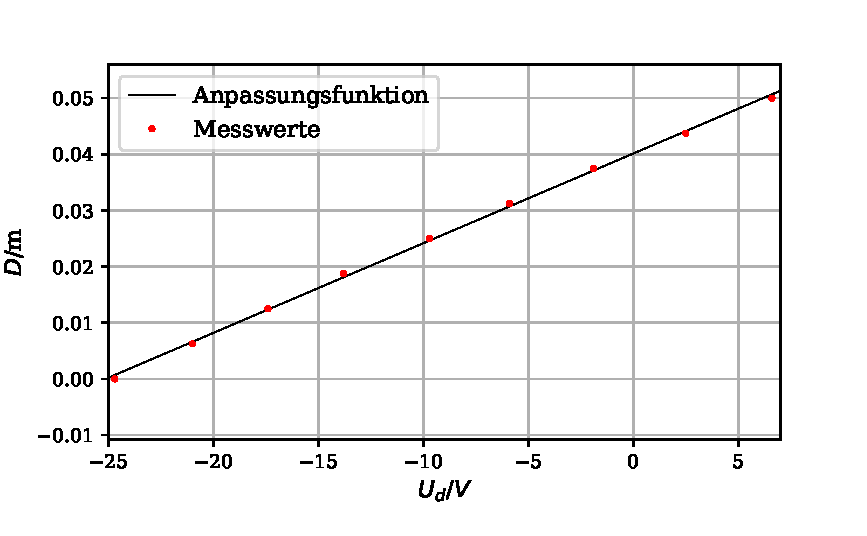
\includegraphics{plot3.pdf}
  \caption{Ablenkung des Strahls in Abhängigkeit von der Ablenkspannung für eine Beschleunigungsspannung von $U_B = 200 \si{\volt}$. }
  \label{fig:plot}
\end{figure}

Der Wert für die Steigung und somit die Empfindlichkeit bei $U_B = 200 \si{\volt}$ lautet
\begin{align*}
\frac{D}{U_D} = (1,597 \pm 0,019) \cdot 10^{-3} \symup{\frac{m}{V}} .
\end{align*}



\begin{table}[H]
  \centering
  \caption{Die gemessene Ablenkspannung und die zugehörigen Ablenkungen bei einer Beschleunigungsspannung von $U_B = 250 \si{\volt}$.}
  \label{tab:Parameter}
  \begin{tabular}{c c}
    \toprule
    $D/$cm& $U_d/$V \\
    \bottomrule
    0,0 & -30,5 \\
     0,625 & -25,6  \\
     1,25 & -21,3 \\
     1,875 & -16,5  \\
     2,5 & -11,9 \\
     3,125 & -6,9  \\
     3,75& -1,7 \\
     4,375 & 2,9  \\
     5,0 &  8,2 \\
     \bottomrule
  \end{tabular}
\end{table}

\begin{figure}[H]
  \centering
  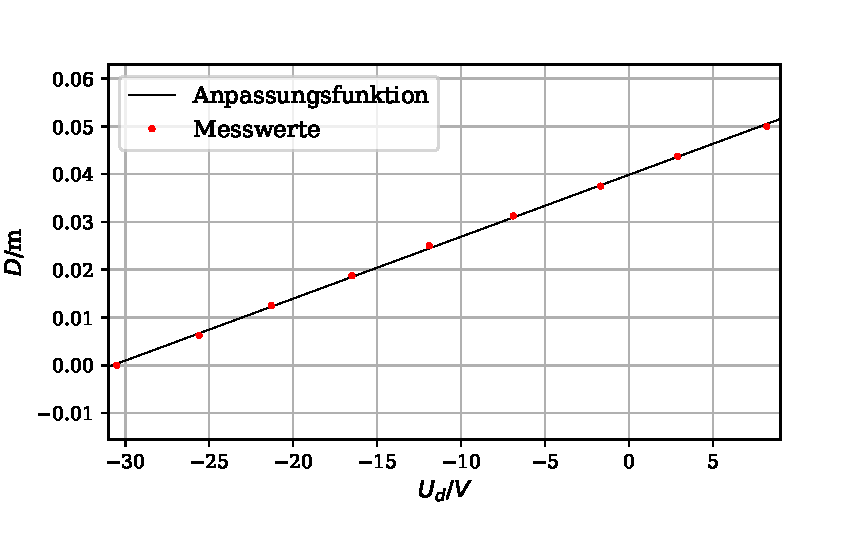
\includegraphics{plot4.pdf}
  \caption{Ablenkung des Strahls in Abhängigkeit von der Ablenkspannung für eine Beschleunigungsspannung von $U_B = 250 \si{\volt}$. }
  \label{fig:plot}
\end{figure}

Der Wert für die Empfindlichkeit bei $U_B = 250 \si{\volt}$ lautet
\begin{align*}
\frac{D}{U_D} = (1,297 \pm 0,011) \cdot 10^{-3} \symup{\frac{m}{V}} .
\end{align*}

\begin{table}[H]
  \centering
  \caption{Die gemessene Ablenkspannung und die zugehörigen Ablenkungen bei einer Beschleunigungsspannung von $U_B = 300 \si{\volt}$.}
  \label{tab:Parameter}
  \begin{tabular}{c c}
    \toprule
    $D/$cm& $U_d/$V \\
    \bottomrule
    0,0 & -36,2 \\
     0,625 & -30,2  \\
     1,25 & -24,8 \\
     1,875 & -19,2  \\
     2,5 & -13,1 \\
     3,125 & -7,6  \\
     3,75& -1,3 \\
     4,375 & 4,8  \\
     5,0 &  10,8 \\
     \bottomrule
  \end{tabular}
\end{table}

\begin{figure}[H]
  \centering
  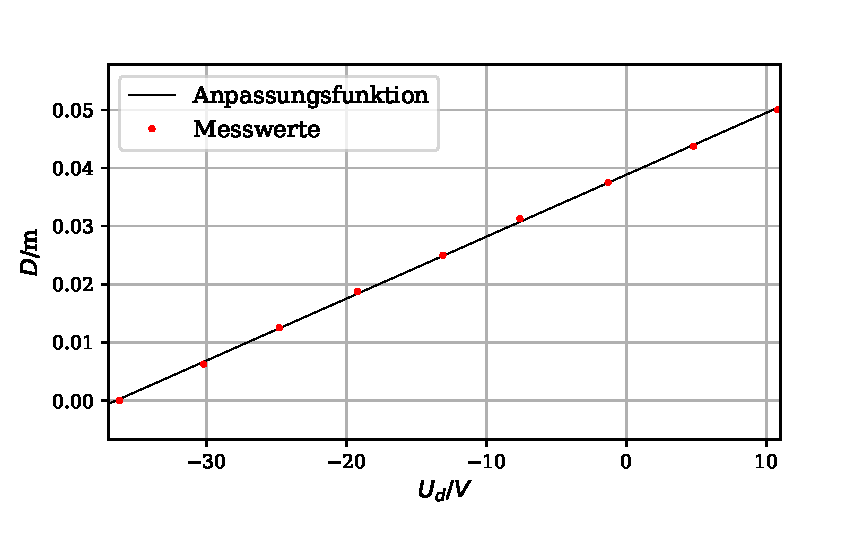
\includegraphics{plot5.pdf}
  \caption{Ablenkung des Strahls in Abhängigkeit von der Ablenkspannung für eine Beschleunigungsspannung von $U_B = 300 \si{\volt}$. }
  \label{fig:plot}
\end{figure}

Der Wert für die Empfindlichkeit bei $U_B = 300 \si{\volt}$ lautet
\begin{align*}
\frac{D}{U_D} = (1,067 \pm 0,008) \cdot 10^{-3} \symup{\frac{m}{V}} .
\end{align*}

\begin{table}[H]
  \centering
  \caption{Die gemessene Ablenkspannung und die zugehörigen Ablenkungen bei einer Beschleunigungsspannung von $U_B = 350 \si{\volt}$.}
  \label{tab:Parameter}
  \begin{tabular}{c c}
    \toprule
    $D/$cm& $U_d/$V \\
    \bottomrule
     0,625 & -35,3  \\
     1,25 & -28,4 \\
     1,875 & -22,1  \\
     2,5 & -15,3 \\
     3,125 & -8,6  \\
     3,75& -1,4 \\
     4,375 & 5,7  \\
     5,0 &  12,4 \\
     \bottomrule
  \end{tabular}
\end{table}

\begin{figure}[H]
  \centering
  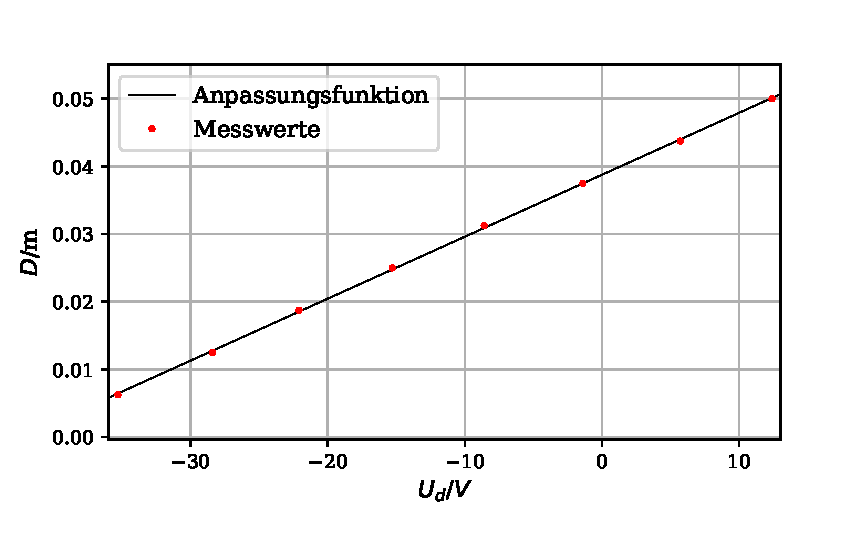
\includegraphics{plot6.pdf}
  \caption{Ablenkung des Strahls in Abhängigkeit von der Ablenkspannung für eine Beschleunigungsspannung von $U_B = 350 \si{\volt}$. }
  \label{fig:plot}
\end{figure}

Der Wert für die Empfindlichkeit bei $U_B = 350 \si{\volt}$ lautet
\begin{align*}
\frac{D}{U_D} = (0,916 \pm 0,006) \cdot 10^{-3} \symup{\frac{m}{V}} .
\end{align*}

\begin{table}[H]
  \centering
  \caption{Die gemessene Ablenkspannung und die zugehörigen Ablenkungen bei einer Beschleunigungsspannung von $U_B = 400 \si{\volt}$.}
  \label{tab:Parameter}
  \begin{tabular}{c c}
    \toprule
    $D/$cm& $U_d/$V \\
    \bottomrule
     0,625 & -37,7 \\
     1,25 & -31,6 \\
     1,875 & -24,1  \\
     2,5 & -16,4 \\
     3,125 & -8,6  \\
     3,75& -0,8 \\
     4,375 & 7,3  \\
     5,0 &  15,0 \\
     \bottomrule
  \end{tabular}
\end{table}

\begin{figure}[H]
  \centering
  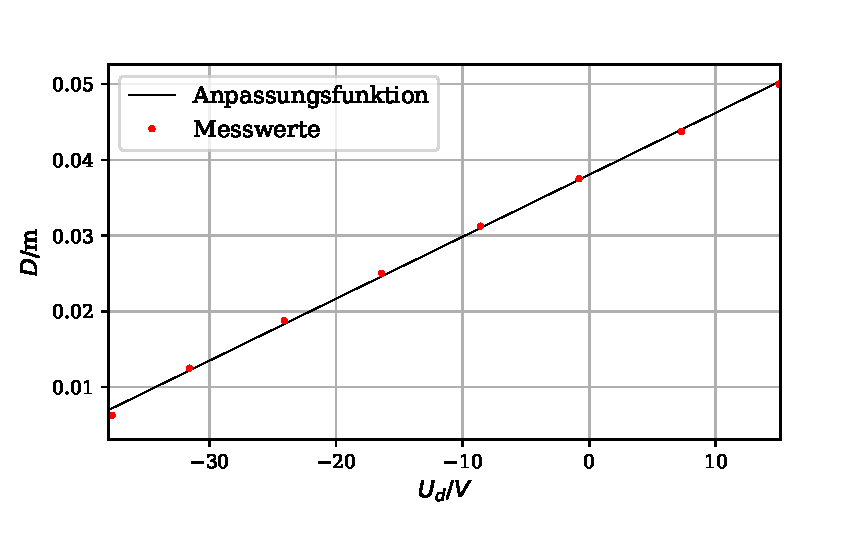
\includegraphics{plot7.pdf}
  \caption{Ablenkung des Strahls in Abhängigkeit von der Ablenkspannung für eine Beschleunigungsspannung von $U_B = 400 \si{\volt}$. }
  \label{fig:plot}
\end{figure}

Der Wert für die Empfindlichkeit bei $U_B = 400 \si{\volt}$ lautet
\begin{align*}
\frac{D}{U_D} = (0,818 \pm 0,010) \cdot 10^{-3} \symup{\frac{m}{V}} .
\end{align*}

\noindent Die Empfindlichkeiten werden nun gegen $\frac{1}{U_B}$ aufgetragen und es wird erneut eine lineare Ausgleichsrechnung durchgeführt. Diese ist in Abbildung (11) zu sehen.

\begin{figure}[H]
  \centering
  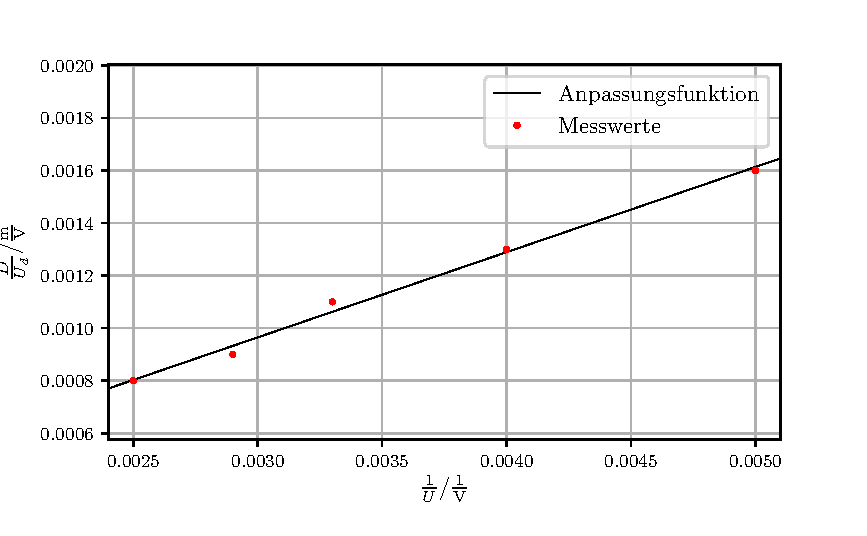
\includegraphics{plot8.pdf}
  \caption{Die berechneten Empfindlichkeiten in Abhängigkeit von $\frac{1}{U_B}$.}
  \label{fig:plot}
\end{figure}

\noindent Die Steigung $a$ dieser Gerade beträgt
\begin{align*}
a = (0,324 \pm 0,015)  \si{\meter} .
\end{align*}

\noindent Berechnet man aus den oben aufgeführten Werten für $p$, $L$ und $d$ den Wert für $\frac{pL}{2d}$, ergibt sich
\begin{align*}
\frac{pL}{2d} = 0,3575 \si{\meter}.
\end{align*}




\subsection{Bestimmung der Frequenz der Sinusspannung aus den gemessenen Synchronisationsfrequenzen}

In Tabelle (6) sind die gemessenen Frequenzen für die Sägezahnspannung aufgelistet, welche bei einer Beschleunigungsspannung von $U_B = 300 \si{\volt}$ gemessen wurden.
Aus Gleichung (4) lässt sich erkennen, dass die Frequenz der Sinusspannung ca. $\nu_{Si} = (50,018 \pm 0,016) \si{\hertz}$ beträgt.
Der Mittelwert der Sinusfreqzenz beträgt
\begin{align*}
\nu_{SiMittel} = \frac{1}{4}\cdot \sum_{n=1}^4 \nu_{Si} = 50,018 .
\end{align*}
Der zugehörige Fehler berechnet sich zu
\begin{align*}
\Delta\nu_{SiMittel} = \frac{1}{\sqrt{4}} \cdot \sqrt{\frac{1}{3} \sum_{n=1}^4 (\nu_{Si,n} - \nu_{SiMittel,n})^2} = 0,016 .
\end{align*}

\noindent Der Scheitelwert berechnet sich aus Formel (3) zu
\begin{align*}
U_d = (11,6 \pm 0,5) \si{\volt} ,
\end{align*}
wobei der Fehler folgendermaßen berechnet wurde:
\begin{align*}
\Delta U_d = \sqrt{(\frac{dU_d}{da})^2\Delta a^2} = 0,5 ,
\end{align*}
mit $\Delta a$ als Fehler von $a$.

\begin{table}[H]
  \centering
  \caption{Frequenzen der Sägezahnspannung und der Sinusspannung in Abhängigkeit von $n$.}
  \label{tab:Spannungsamplitude}
  \begin{tabular}{c c c}
    \toprule
    $n$ & $\nu_{Sa} / \symup{\frac{1}{s}}$ & $\nu_{Si} / \symup{\frac{1}{s}}$\\
    \midrule
    1/2 &  25,01 & 50,02 \\
      1 &  50,02 & 50,02 \\
      2 & 100,03 & 50,015 \\
      3 & 150,05 & 50,017\\
    \bottomrule
  \end{tabular}
\end{table}

\noindent Die gemessene Strahlauslenkung beträgt $s = 0,0125 \si{\m} $.

























\subsection{Bestimmung der spezifischen Ladung der Elektronen}
In Tabelle (7) sind die Strahlverschiebungen $D$ und die jeweiligen Stromstärken $I$ angegeben.


\begin{table}[H]
  \centering
  \caption{Stromstärke der Helmholtz-Spule und die zugehörigen Ablenkungen bei einer Beschleunigungsspannung von $U_B = 250 \si{\volt}$.}
  \label{tab:Parameter}
  \begin{tabular}{c c}
    \toprule
    $D/$cm& $I/$A \\
    \bottomrule
    0,0 & 0,0 \\
     0,625 & 0,3  \\
     1,25 & 0,65 \\
     1,875 & 1,0  \\
     2,5 & 1,3 \\
     3,125 & 1,65  \\
     3,75& 1,95  \\
     4,375 & 2,3  \\
     5,0 &  2,65 \\
     \bottomrule
  \end{tabular}
\end{table}

\noindent In einem Diagramm wird die Größe $\frac{D}{(L^2+D^2)}$ gegen das Magnetfeld $B$ aufgetragen.
Um das Magnetfeld auszurechnen, benötigt man laut Gleichung (8) folgende Größen: Die Windungszahl der Spule $N=20$ und ihren Radius $R=28,2$\si{\cm}, und
den Weg $L=17,5$ \si{\cm}, welcher von der Beschleunigungselektrode bis zum Leuchtschirm reicht.
Die für den Plot notwendigen Werte sind in Tabelle (8) aufgeführt.
\begin{equation}
B = \mu_0 \frac{8NI}{\sqrt{125}R}
\end{equation}
  


\begin{table}[H]
  \centering
  \caption{Berechnetes Magnetfeld und die Größe $D/(L^2+D^2)$ bei einer Beschleunigungsspannung von $U_B = 250 \si{\volt}$.}
  \label{tab:Parameter}
  \begin{tabular}{c c}
    \toprule
    $\frac{D}{(L^2+D^2)}$& $ $B$ \cdot 10^{-5} /$T \\
    \bottomrule
     0,0 & 0,0 \\
     0,204 & 1,913  \\
     0,406 & 4,146 \\
     0,605 & 6,378 \\
     0,800 & 8,290 \\
     0,989 & 10,522  \\
     1,171 & 12,435  \\
     1,345 & 14,667 \\
     1,509 & 16,899 \\
     \bottomrule
  \end{tabular}
\end{table}


\begin{figure}[H]
  \centering
  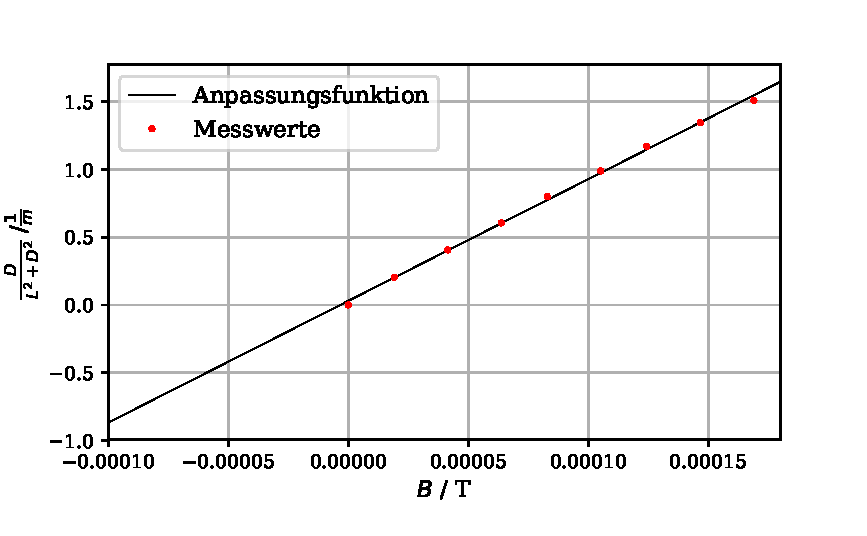
\includegraphics{plot1.pdf}
  \caption{Die Größe $D/(L^2+D^2)$ aufgetragen gegen das Magnetfeld bei einer Beschleunigungsspannung von $U_B = 250\si{\volt}$.}
  \label{fig:plot}
\end{figure}

Die lineare Ausgleichsrechnung $y = mx+C$ hat die Form
\begin{align*}
    \frac{D}{(L^2+D^2)} = \frac{1}{\sqrt{8U_B}}\sqrt{\frac{e_0}{m_0}} \cdot B + C .
\end{align*}

Es ergeben sich die Parameter
\begin{align*}
    m = (8,98 \pm 0,14) \cdot 10^{3} \symup{\frac{1}{T}},\\
    C = (3,01 \pm 1,42) \cdot 10^{-2} .
\end{align*}

Aus der Steigung berechnet man mit Hilfe von Formel (7) den Wert für $\frac{e_0}{m_0}$ :
\begin{align*}
\frac{e_0}{m_0} = (1.61 \pm 0.05) \cdot 10^{11} \symup{\frac{C}{kg}}.
\end{align*}

\noindent Die Gleiche Rechnung wird für eine Beschleunigungsspannung von $U_B = 435\si{\volt}$ durchgeführt. Die Messwerte dazu und die benötigten Werte für den Plot sind in Tabelle (9) aufgelistet.

\begin{table}[H]
  \centering
  \caption{Stromstärke der Helmholtz-Spule, die zugehörigen Ablenkungen, das berechnete Magnetfeld und die Größe $D/(L^2+D^2)$ bei einer Beschleunigungsspannung von $U_B = 435 \si{\volt}$.}
  \label{tab:Parameter}
  \begin{tabular}{c c c c}
    \toprule
    $D/$cm& $I/$A & $\frac{D}{(L^2+D^2)}$ & $ $B$ \cdot 10^{-5} /$T\\
    \bottomrule
    0,0 & 0,0 & 0,0 & 0,0\\
    0,625 & 0,4 & 0,204 & 2,551 \\
    1,250 & 0,8 & 0,406 & 5,102\\
    1,875 & 1,2 & 0,605 & 7,653\\
    2,50 & 1,65 & 0,800 & 10,522\\
    3,125 & 2,05 & 0,989 & 13,073\\
    3,750 & 2,5 & 1,171 & 15,942\\
    4,375 & 2,95 & 1,345 & 18,813\\
    5,0 & 3,35 & 1,509 & 21,363\\
    
     \bottomrule
  \end{tabular}
\end{table}

Der zugehörige Plot ist in Abbildung (13) zusehen.


\begin{figure}[H]
  \centering
  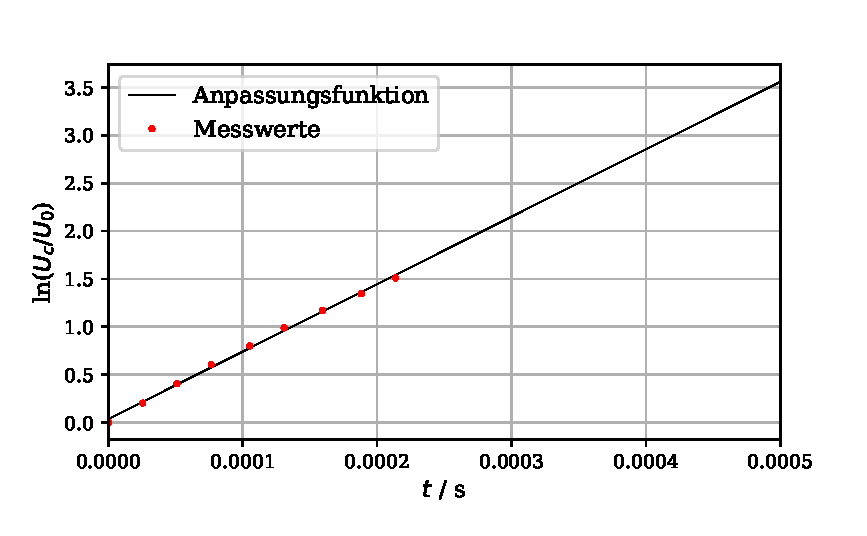
\includegraphics{plot2.pdf}
  \caption{Die Größe $D/(L^2+D^2)$ aufgetragen gegen das Magnetfeld bei einer Beschleunigungsspannung von $U_B = 435\si{\volt}$}
  \label{fig:plot}
\end{figure}

Aus der Ausgleichsrechnung ergeben sich die Parameter
\begin{align*}
    m = (7,04 \pm 0,13) \cdot 10^{3} \symup{\frac{1}{T}},\\
    C = (3,74 \pm 1,68) \cdot 10^{-2} .
\end{align*}

Der Wert für $\frac{e_0}{m_0}$ ergibt sich zu
\begin{align*}
\frac{e_0}{m_0} = (1.72 \pm 0.06) \cdot 10^{11} \symup{\frac{C}{kg}}.
\end{align*}


\subsection{Bestimmung der Intensität des lokalen Erdmagnetfeldes}
Die Stromstärke wurde gemessen und beträgt $I = 0,15$ \si{\ampere}.
Laut Gleichung (8) ergibt sich daraus eine Magnetfeldstärke von
\begin{align*}
    B = 9,566 \cdot 10^{-6} \si{\tesla}.
\end{align*}
Der gemessene Inklinationswinkel beträgt $\phi = 80°$.
Die Totalintensität des Erdmagnetfelds beträgt also
\begin{align*}
    B_{total} = \frac{B}{cos(\phi)} = -8,666 \cdot 10^{-5} \si{\tesla}.
\end{align*}
